\subsection{Patchplot Library}
\label{sec:lib:patchplots}
\begin{pgfplotslibrary}{patchplots}
	A library for advanced |patch| plots. It has been designed to visualize shaded isoparametric finite element meshes of higher order. Its core is an interface to the generation of smoothly shaped elements which are shaded bilinearly (\texttt{.pdf} Shading Type 6 and \texttt{.pdf} Shading Type 7), with additional (limited) support for constant color filling without shadings.

\begin{pgfplotskey}{patch type=\mchoice{default,rectangle,triangle,line,bilinear,triangle quadr,biquadratic,coons} (initially default)}
	The |patchplots| library supports several new |patch type|s in addition to the initially available choices (which are |rectangle|,|triangle| and |line|). The documentation of these choices are replicated from page~\pageref{key:patch:type} here.

	The |patchplots| library is especially strong for |shader=interp|, so this is our main focus in the documentation here.

	\paragraph{Attention:} At the time of this writing, many free pdf viewers do not fully support the following shadings\footnote{The author of this package has submitted bugfixes to Linux viewers based on xpdf/libpoppler, so the problem will vanish in the future versions.}. The preferred viewer is Adobe Acrobat Reader.

	The choice \declaretext{rectangle} expects one or more rectangular patches with $n=4$ vertices each. These vertices are either encoded as a matrix or as individual patches (using |mesh input=patches|), in the sequence in which you would connect the vertices:
\begin{codeexample}[]
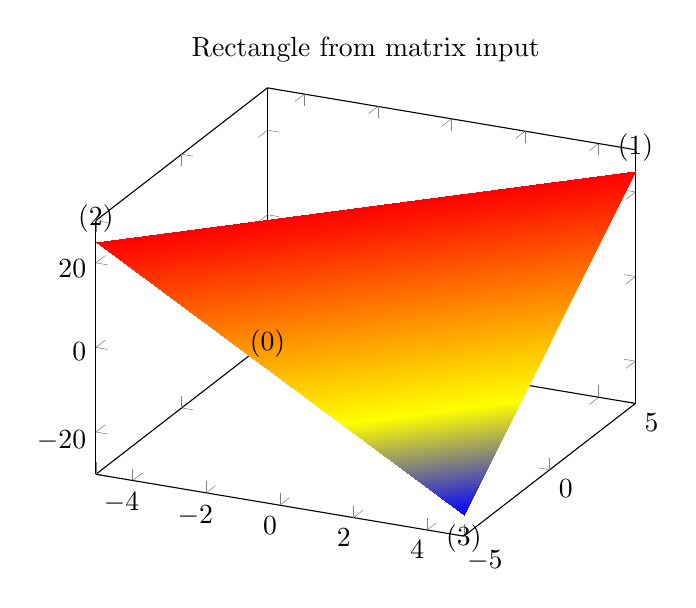
\begin{tikzpicture}
	\begin{axis}[nodes near coords={(\coordindex)},
		title=Rectangle from matrix input]
	% note that surf implies 'patch type=rectangle'
	\addplot3[surf,shader=interp,samples=2,
		patch type=rectangle] 
		{x*y};
	\end{axis}
\end{tikzpicture}
\end{codeexample}
\begin{codeexample}[]
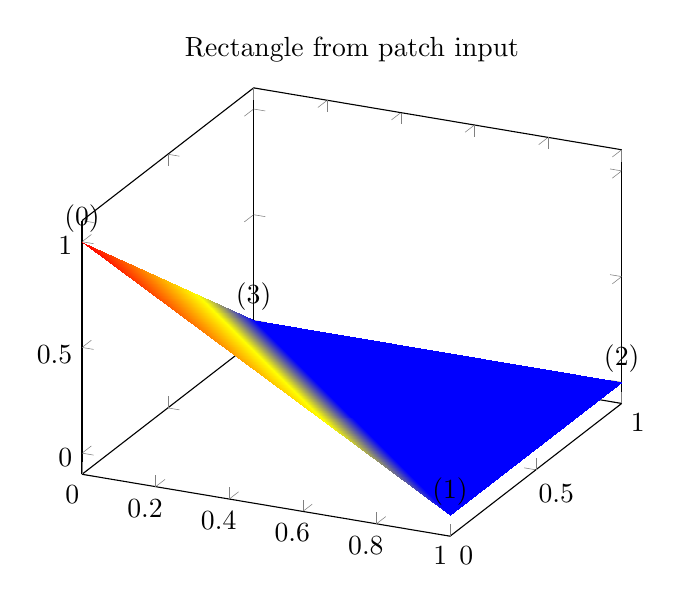
\begin{tikzpicture}
	\begin{axis}[nodes near coords={(\coordindex)},
		title=Rectangle from patch input]
	\addplot3[patch,shader=interp,patch type=rectangle] coordinates {
		(0,0,1) (1,0,0) (1,1,0) (0,1,0)
	};
	\end{axis}
\end{tikzpicture}
\end{codeexample}
	\noindent As already documented on page~\pageref{key:patch:type}, the |shader=interp| implementation for |rectangle| uses two triangles and interpolates them linearly.

	The choice \declareandlabel{bilinear} is essentially the same as |rectangular| with respect to its input formats and stroke paths, but it uses correct bilinear shading for |shader=interp|. The two examples from above now become
\begin{codeexample}[]
\begin{tikzpicture}
	\begin{axis}[nodes near coords={(\coordindex)},
		title=Bilinear from matrix input]
	% note that surf implies 'patch type=rectangle'
	\addplot3[surf,shader=interp,samples=2,
		patch type=bilinear] 
		{x*y};
	\end{axis}
\end{tikzpicture}
\end{codeexample}
\begin{codeexample}[]
\begin{tikzpicture}
	\begin{axis}[nodes near coords={(\coordindex)},
		title=Bilinear from patch input]
	\addplot3[patch,shader=interp,patch type=bilinear] coordinates {
		(0,0,1) (1,0,0) (1,1,0) (0,1,0)
	};
	\end{axis}
\end{tikzpicture}
\end{codeexample}

	The choice \declaretext{triangle} expects a sequence of linear triangles, each encoded using $n=3$ vertices:
\begin{codeexample}[]
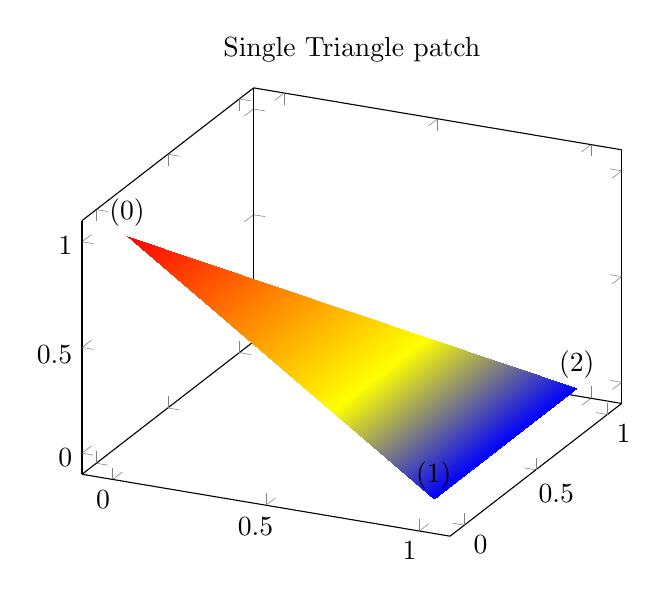
\begin{tikzpicture}
\begin{axis}[enlargelimits,
	nodes near coords={(\coordindex)},
	title=Single Triangle patch]
\addplot3[patch,shader=interp] coordinates {
	(0,0,1)
	(1,0,0)
	(1,1,0)
};
\end{axis}
\end{tikzpicture}
\end{codeexample}

	The choice \declareandlabel{triangle quadr} expects a sequence of isoparametric quadratic triangles, each defined by $n=6$ vertices:
\begin{codeexample}[]
\begin{tikzpicture}
	\begin{axis}[nodes near coords={(\coordindex)},
		title=Quadratic Triangle]
	\addplot3[patch,patch type=triangle quadr,shader=interp]
	coordinates {
		(0,0,1)	(5,4,0)	(0,7,0)
		(2,3,0) (3,6,0) (-1,4,0)
	};
	\end{axis}
\end{tikzpicture}
\end{codeexample}
	\noindent Here, the edges have the correct quadratic shape, represented as second order Bezier curves.
\end{pgfplotskey}

\begin{pgfplotskey}{patch refines=\marg{integer} (initially 0)}
	
\end{pgfplotskey}

\begin{pgfplotskey}{patch to triangles=\mchoice{true,false} (initially false)}
	
\end{pgfplotskey}

\end{pgfplotslibrary}
